% -*- mode: LaTeX; coding: utf-8; -*-

\chapter{Web-palveluiden haasteet}

Toimivan ja ennen kaikkea turvallisen web-pohjaisen palvelun tarjoaminen vaatii
nykyisin paljon enemmän huomiota ja aikaa niin palvelun kehittäjältä kuin myös
palvelun tarjoajalta ja ylläpitäjältä kuin ennen. Ajat ovat muuttuneet siitä,
jolloin käyttäjät selailivat pääasiassa staattisia web-sivuja, ja käyttivät
palveluista korkeintaan sähköpostia. Kehitys kulkee kovaa vauhtia eteenpäin, ja
tämän päivän suurimpia villityksiä ovat asiat kuten interaktiivisuus,
sosiaalisuus ja yksilöllisyys, joiden kautta verkon käytöstä pyritään tekemään
käyttäjälle entistä henkilökohtaisempi kokemus. Palvelut kuten MySpace,
Facebook ja YouTube ovat edelleen vahvistaneet näitä käyttäjätottumuksia, ja
markkinoille onkin syntynyt kova kilpailu siitä, kuka kehittää seuraavan
hittipalvelun. Nykyisin puhutaankin internetin seuraavasta evoluutiosta Web 2.0:
n muodossa, joita myös edellä mainitut palvelut edustavat. Uudet teknologiat ja
kiire tuovat kuitenkin aina mukanaan joukon uusia heikkouksia, joita hyökkääjät
pyrkivät hyödyntämään. Ylläpitäjien kannalta onkin tärkeää, että kehityksen
tuomiin haasteisiin pyritään vastaamaan mahdollisimman nopeasti ja tehokkaasti.

\section{Mitä tarkoittaa Web 2.0?}

Web 2.0 on termi, jota käytetään hyvin monessa eri tarkoituksessa ja
asiayhteydessä. Se yhdistetään usein mm. uuteen web-teknologiaan tai internet-
aikakauden tuotteen/palvelun kehityskaaren esittämiseen \cite{WEB2}. Yhteistä näille
on, että ne pyrkivät kuvaamaan sitä muutosta, jota internet pitää tällä
hetkellä sisällään. Tämä muutos on lähtöisin siitä, että kuluttajatottumukset
ovat kehittyneet kohti interaktiivisia palvelumalleja, joissa käyttäjillä on
suuri vaikutusvalta siihen mitä informaatiota esitetään ja kuinka se esitetään.
Sosiaalisuus ja sen luoma yhteisöllisyys ovat luoneet tarpeen palveluille,
joissa käyttäjät pystyvät tekemään useita asioita samaan aikaan saumattomasti
yhdestä paikasta käsin. Toinen kantava voima muutokselle on markkinoiden tuoma
paine, joka pyrkii mukautumaan muuttuneisiin vaatimuksiin sekä
kuluttajapuolella että yrityspuolella. Tätä varten joudutaan kehittämään yhä
isompia kokonaisuuksia uusilla teknologioilla, joiden käyttöä ei vielä hallita
tarpeeksi. Tähän kun vielä lisätään kiire päästä markkinoilla ensimmäisten
joukossa, niin tietoturva jää usein taka-alalle \cite{WEB2b}.

Tietoturvan kannalta teknologiat, jotka luetaan kuuluvan osaksi Web 2.0
teknologiaperhettä, ovat jatkuvan huomion kohteena. Nämä teknologiat
muodostavat sen voiman, joka mahdollistaa siirtymisen interaktiivisiin
sovelluksiin kuten Google Maps, ja yritysten toiminnan siirtymisen verkkoon.
Teknologiat kuten Asynchronous JavaScript (AJAX), Cascading Style Sheet (CSS),
Flash, ActiveX ja XML voidaan kaikki laskea kuuluvan osaksi Web 2.0-perhettä.
Osa näistä teknologioista on ollut jo pidemmän aikaa käytössä kun taas osaa on
vasta nyt alettu käyttämään siihen, mihin ne alun perin oli suunniteltu \cite{WEB2}.
Kuvassa \ref{web} on nähtävillä näiden yleisimpien teknologioiden ja protokollien
väliset suhteet.

\begin{figure}[htp]
\centering
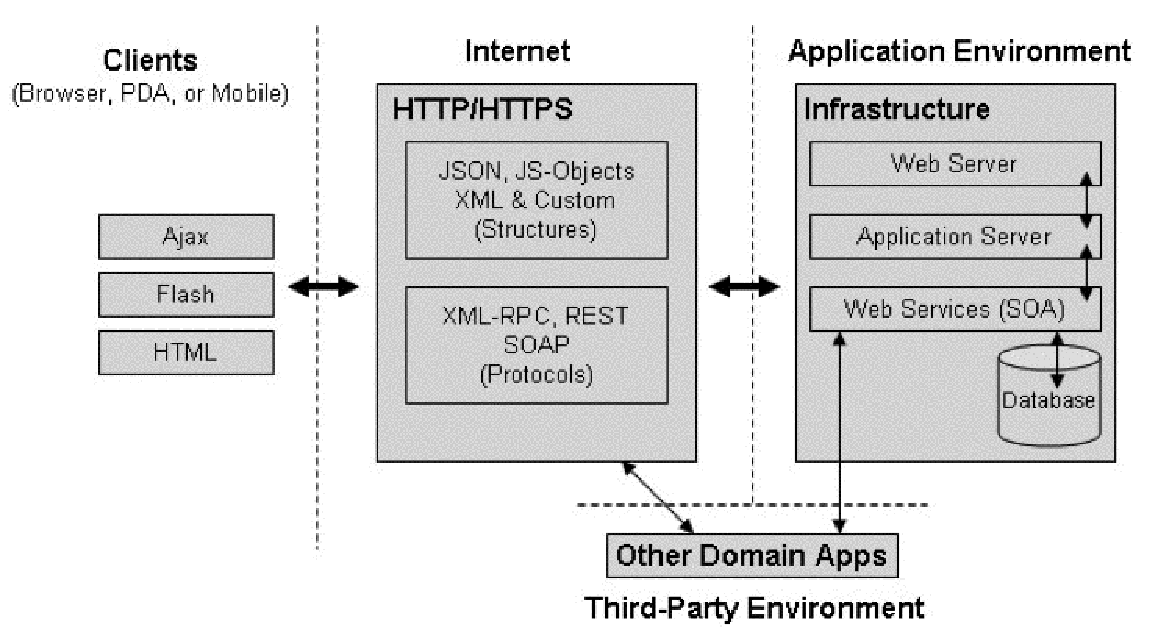
\includegraphics[width=12cm]{pics/web.pdf}
\caption{Web 2.0}
\label{web}
\end{figure}

Mitä Web 2.0 sitten tarkoittaa tietoturvan kannalta? Ensinnäkin sen mukana
tulee samat vanhat haavoittuvuudet kuin mitä Web 1.0 sisälsi. Näiden lisäksi
hyökkäykset kuten Cross-site Scripting (XSS) ja Cross-site Request Forgery (
CSRF) ovat aikaisempaa vaarallisia, koska käytetyt teknologiat mahdollistavat
rikkaamman ympäristön, jonka kautta murtautua järjestelmiin \cite{WEB2}. Web 2.0
sovellukset antavat myös loppukäyttäjälle ja takana oleville ohjelmille enemmän
valtaa, jonka johdosta loppukäyttäjä ei välttämättä edes huomaa joutuessaan
tietomurron kohteeksi. Otetaan esimerkiksi Ajax-teknologia, joka mahdollistaa
sivujen tietojen päivittämisen käyttäen asynkronisia kutsuja. Tämän ansiosta
käyttäjä pystyy tekemään kutsuja palvelimille ja päivittämään osan sivun
tiedoista niin, ettei koko sivua tarvitse päivittää. Tästä suurin osa tapahtuu
käyttäjältä piilossa, joten hän ei todennäköisesti huomaa, jos selain lataa
haitallisia ohjelmia koneelle käyttäen jotain tunnettua haavoittuvuutta.
Arviolta 70 prosenttia kaikista haitallisista koodeista ladataankin käyttäen
Ajaxia \cite{WEB2c}.

Palvelinpuolella muutokset eivät rajoitu vain Web 2.0 tuomiin
tietoturvariskeihin, sillä uudenlainen ajattelu vaatii myös uudenlaisen
palveluarkkitehtuurin. Uusi arkkitehtuuriratkaisu tuo aina mukanaan suuren
joukon muutoksia, jotka tulee ottaa huomioon tietoturvaa suunniteltaessa.
Palvelukeskeinen arkkitehtuuri (engl. Service Oriented Architecture, SOA) on
yksi näistä kehysmalleista, joka on kasvattanut kannatustaan Web 2.0:n
vanavedessä. SOA-arkkitehtuurilla onkin nykyisin tärkeä rooli palvelujen
välisen kommunikoinnin kehittämisessä. Siksi onkin tärkeää ymmärtää mistä
palasista SOA-arkkitehtuuriin perustuvat palvelut koostuvat, ja mitä tämä
tarkoittaa turvallisuuden kannalta.

\section{Palvelukeskeinen arkkitehtuuri}

Web-pohjaiset teknologiat ovat saamassa yhä suurempaa huomiota yrityspuolen
sovelluskehityksessä. Tätä muutosta on ollut ohjaamassa teknologioiden
kehittyminen siihen pisteeseen, jossa yritykset pystyvät tarjoamaan aikaisemmin
asiakas-serveri sovelluksia verkon välityksellä luotettavasti ja nopeasti. Tämä
ratkaisu on tuonut mukanaan rahallisia säästöjä yrityksille, jotka ovat ennen
joutuneet itse huolehtimaan mm. sovellusten ajan tasalla pitämisestä ja
palvelimien ylläpitämisestä \cite{WEB2}. Tämä muutos on luonut myös tarpeen löytää yhä
tehokkaampia kehitysmalleja ja tapoja toteuttaa entistä monimutkaisempia ja
vaativimpia sovelluksia suuryritysten tarpeisiin. Yksi tapa hallita tätä
muutosta on perustaa tehdyt ohjelmistosuunnitelman ratkaisut palvelukeskeisen
arkkitehtuurin malliin.

Puhuttaessa web-palveluista palvelukeskeinen arkkitehtuuri lähtee siitä
ajatuksesta, että palveluiden toiminnot ja prosessit pyritään suunnittelemaan
toimimaan mahdollisimman itsenäisesti ja avoimesti siten, että niitä pystytään
kutsumaan joustavasti eri sovellusten välillä käyttäen standardoitua rajapintaa.
Tähän ratkaisuun on ajanut pyrkimys laskea IT-kustannuksia ja maksimoida jo
käytössä olevien ratkaisujen uudelleenkäyttöä. Aikaisemmin tämän toteuttaminen
on ollut vaikeaa sovellusten heterogeenisyyden takia, jonka johdosta eri
alustojen ja toimittajien väliset yhteistoiminnot ovat olleet usein mahdottomia
toteuttaa. Yhä useamman sovelluksen ja palvelun siirtyessä verkkoon tästä
halutaan nyt päästä eroon, ja tähän ongelmaan palvelukeskeinen arkkitehtuuri
pyrkii tuomaan ratkaisun. Käytännössä tämä tarkoittaa sitä, että arkkitehtuurin
tulee tarjota sovelluksille mahdollisimman joustavan sekä sijainnista ja
protokollasta riippumattoman alustan \cite{SOA}. Tämän avulla loppukäyttäjälle
voidaan tarjota palveluita monesta eri paikasta yhtä aikaa siten, ettei hän ole
tästä edes tietoinen. Kyseessä on sama ajattelumalli johon Web 2.0 sovellukset
pohjautuvat, ja siksi palvelukeskeinen arkkitehtuuri onkin saanut paljon
nostetta Web 2.0:n myötä.

Palvelukeskeisen arkkitehtuurin tuomat edut eivät rajoitu pelkästään
kustannussäästöihin. Sen tuomiin etuihin kuuluu myös mm. uusien toimintojen
helpompi integrointi jo käytössä oleviin järjestelmiin sekä monimutkaisten
kokonaisuuksien helpompi hallinta. Organisaatiolle on myös tärkeää, että tällä
tavalla suunniteltuun palvelumalliin muutoksia on nopeampi tehdä ja reagointi
markkinamuutoksiin voidaan toteuttaa nopeassa aikataulussa \cite{WEB2c}. Tämä on
erityisen tärkeää, koska markkinoille on ilmestynyt monia uusia tekniikoita,
jotka mahdollistavat web-palveluiden integroinnin jo käytössä oleviin
palveluihin. Onkin arvioitu, että vuonna 2008 web-pohjaisiin palveluihin
käytettiin jo yli 11 miljardia dollaria, ja osa fokuksesta on jo siirtynyt
kohti keskikokoisia ja pieniä yrityksiä. Web-pohjaisten palveluiden merkityksen
uskotaankin entisestään kasvavan ja yritykset, jotka eivät reagoi tähän
muutokseen, huomaavat tulevaisuudessa olevansa epäsuotuisassa asemassa \cite{WEB2b}.

Palvelinpuolelle tapahtuva muutos tarkoittaa sopeutumista uudenlaiseen
ajattelumalliin, jossa palvelut on hajautettu ympäri verkkoa, ja joista osa ei
välttämättä ole saman ylläpitäjän hallinnassa. Kuvan \ref{soa} mukainen ratkaisu
tulee olemaan tulevaisuudessa arkipäivää, ja se tuo mukanaan uusia rajapintoja,
joiden kautta hyökkääjä voi pyrkiä murtautumaan järjestelmään tai jopa
yrityksen sisäiseen verkkoon. Koska palveluiden välinen kommunikointi perustuu
tässä mallissa luottamussuhteen luomiseen, tulee erityistä kiinnittää huomiota
siihen kuinka salaukset ja tunnistautuminen hoidetaan web-palveluita tarjoavien
osapuolien sekä käyttäjien kesken \cite{WEB2b}.

\begin{figure}[htp]
\centering
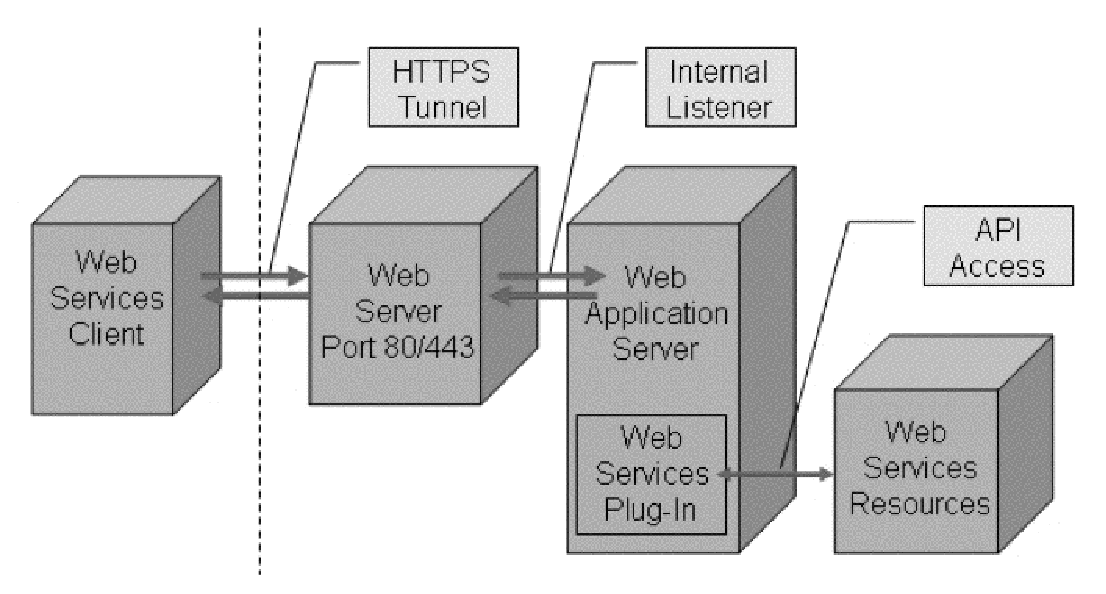
\includegraphics[width=12cm]{pics/soa.pdf}
\caption{SoA-arkkitehtuuri}
\label{soa}
\end{figure}

\section{Web-palveluiden tietoturva}

Internetin kehittyessä myös web-palveluihin kohdistuvat hyökkäykset ovat saaneet
uusia ilmenemismuotoja. Aikaisemmin ``web hakkerointia'' käytettiin kuvaamaan
hyökkäyksiä, jotka kohdistuivat palveluita tarjoaviin alustoihin kuten Apache, 
Microsoft IIS ja LAMP. Nämä hyökkäykset perustuivat tunnettujen haavoittuvaisuuksien
hyödyntämiseen, ja oikeille työkaluilla varustautunut hyökkääjä pystyikin kaatamaan haavoittuvan
palvelun muutamassa minuutissa. Esimerkiksi tunnetuimpien internet-matojen Code Redin ja Nimdan toiminta
perustui Microsoft IIS:sä olevan haavoittuvuuden hyödyntämiseen \cite{Hacking}. 

Tämänlaiset hyökkäykset ovat kuitenkin
menettäneet suurimman tehonsa, koska tehdyistä virheistä on opittu. Löydettyihin haavoittuvaisuuksiin
reagoidaan entistä nopeammin, yhä useampi alusta on konfiguroitu oikein ja saatavilla on työkaluja, joiden
avulla pystytään nopeasti ja helposti havaitsemaan yleisimmät tietoturvariskit \cite{Hacking}. Näistä seikoista johtuen
hyökkääjät ovatkin kiinnittäneet entistä enemmän huomiota itse alustalla pyöritettäviin palveluihin pyrkien 
murtautumaan järjestelmiin näiden kautta. Web 2.0:n myötä tämän tyyppiset hyökkäykset ovat saaneet entistä
enemmän huomiota, sillä se on tarjonnut hakkereille entistä monipuolisemman hyökkäyspinnan. Tietoturvan 
kannalta onkin tärkeää, että kumpaankin hyökkäystyyppiin kiinnitetään huomiota.

\subsection{Web-palvelimien turvaaminen}

Yllä mainitut seikat eivät tarkoita sitä, että web-palveluita pyörittävät alustat olisivat
turvassa hyökkäyksiltä. Onnistuneet hyökkäykset ovat edelleen yhtä tuhoisa, jos niihin ei ole ennalta 
varauduttu. Nämä erilaiset hyökkäykset pyrkivät yleensä hyödyntämään seuraavissa kategorioissa olevia heikkouksia

\begin{itemize}
\item Valmiit esimerkkitiedostot
\item Lähdekoodin paljastuminen
\item Kanonisointi
\item Palvelmiin asennetut lisäosat
\item Syötteen tarkistaminen \cite{Hacking}.
\end{itemize}

Näiltä suojautuminen on melko yksinkertaista, kunhan muistaa noudattaa muutamaa pääperiaatetta. Ensinnäkin tuotannossa 
olevilla palvelimilla ei tulisi koskaan olla asennettuna tai käytettynä tiedostoja, joiden turvallisuudesta ei ole
takeita. Näihin tiedostoihin kuuluvat mm. paketeissa mukana tulleet esimerkkitiedostot ja palvelimelle asennettavat 
lisäosat, joiden alkuperästä ei ole varmuutta. Toisekseen on tärkeää varmistaa, että käytettyihin sovelluksiin
on asennettu viimeisimmät päivitykset, sillä nämä yleensä korjaavat tunnetut heikkoudet \cite{Hacking}. Jo pelkästään näillä 
toimilla pystytään suurimmaksi osaksi estämään palvelmiin kohdistuvat hyökkäykset. 

\subsection{SQL injektio}

Virheelliseen syöttötietoon perustuvat hyökkäykset ovat jo pidemmän aikaa vaivanneet web-pohjaisia sovelluksia.
Web 2.0:n myötä hyökkäykset ovat entisestään yleistyneet, sillä monimutkaisten sovellusten takana käytetään entistä
enemmän erilaisia tietokantapohjaisia ratkaisuja kuten MySQL. Nämä hyökkäykset hyödyntävät sitä seikkaa, että suurin osa
sovelluksista ei tee selkeää eroa käyttäjän antaman syötteen ja ohjelmalle annettavien ohjeiden välillä. Tämä mahdollistaa
sen, että hyökkääjä pystyy piilottamaan annettuun hakuun ohjelmatason käskyjä, jotka muokkaavat sovelluksen toimintaa
hyökkääjän haluamaan suuntaan \cite{WEB2}. Normaaleilla toimenpiteillä tällaisen hyökkäysten tunnistaminen on hankalaa, sillä
yritysten tietoturvasta vastaavat palomuurit toimivat OSI-mallin kolmannella, neljännellä ja viidennellä kerroksella, eivätkä ne tunnista
ylimmän tason eli ohjelmistotason kautta tulevia hyökkäyksiä. Tämän lisäksi useimmat palomuurit eivät ymmärrä protokollien
kuten HTTP:n tarkkaa sisältöä \cite{SQL SS}.    

Onnistunut injektiohyökkäys koostuu kolmesta erillisestä vaiheesta. Ensimmäisessaä vaiheessa hyökkääjän tulee tunnistaa 
web-sovelluksessa käytetyt teknologiat. Tämä onnistuu mm. tulkitsemalla sivujen antamia virheilmoituksia, tutkimalla 
sivun lähdekoodia tai käyttäen tätä varten tehtyjä työkaluja kuten Nessus ja Nmap. Tämä vaihe on hyökkääjälle melko triviaali
tehtävä, mutta hyökkäyksen kannalta tiedot ovat elintärkeitä, sillä injektiohyökkäyksen onnistuminen on täysin riippuvainen 
käytetystä ohjelmointikielestä. Kun tarvittavat tiedot on saatu kerättyä, voidaan varsinaista hyökkäystä alkaa suunnittelemaan.
Tämä tapahtuu tunnistamalla ne syötteet, jotka käyttäjä pystyy sovellukselle antamaan. Tämä käsittää käytännössä kaiken sen 
datan, joka kulkee HTTP GET ja HTTP POST pyynnöissä. Viimeisessä vaiheessa hyökkääjän tehtäväksi jää sitten niiden syötteiden 
tunnistaminen, joita käyttämällä sovelluksen toiminta saadaaan muokattua. Tähänkin tehtävään löytyy useita työkaluja, ja
monessa tapauksessa samat periaatteet toimivat eri sovellusten välillä \cite{WEB2}.

Structured Query Language (lyh. SQL), joka on alan de facto standardi tietokantojen käsittelyyn, on käytössä lähes jokaisessa
web-sovelluksessa, joka käyttää jonkinlaista tietokantaratkaisua. Sen syntaksi on sekoitus ohjelmakäskyjä ja käyttäjän antamia
syötteitä, ja huonosti määritettynä käyttäjän antama syöte voidaan tulkita virheellisesti ohjelmatason käskyksi. Tämän syötteen
hyökkääjä joutuu usein etsimään sokeasti, mutta syötteet kuten

\begin{itemize}
\item ' OR 1=1 "{-}{-}
\item ') OR 1=1 "{-}{-}
\end {itemize}
\linebreak
toimivat hyvin usein \cite{WEB2}. Virheellisestä hausta aiheutuvat virheilmoitukset antavat myös erittäin paljon
hyödyllistä tietoa hyökkääjälle \cite{SQL SS}. Koska suurin osa SQL-tietokannoista mahdollistaa useamman perättäisen syötteen 
antamisen, kunhan syntaksi pysyy oikeana, voidaan näiden avulla katkaista ohjelman normaali toiminta. Otetaan esimerkiksi SQL-haku
\begin{center}\tt
String query= ``SELECT id FROM user\_table WHERE `` + \\
``username = ' `` + username + ``' AND `` + \\
``password = PASSWORD(' `` + password + ``')''; \\
\end{center}
\end{tt}
\linebreak
Antamalla käyttäjänimeksi arvon

\begin{center}\tt
' OR 1=1; DROP TABLE user\_table;"{-}{-}
\end{center}
\end{tt}
\linebreak
muuttuu tietokannalle ohjautuva kysely muotoon

\begin{center}\tt
String query= ``SELECT id FROM user\_table WHERE username=' ' OR 1=1; DROP TABLE
user\_table; "{-}{-} ' AND password = PASSWORD ('x');
\end{center}
\end{tt}
\linebreak
SQL-kielessä kaksi perättäistä viivaa tarkoittaa, että kaikki siitä oikealla puolella oleva on kommenttia. 
Näin ollen lopullinen SQL-haku on 

\begin{center}\tt
String query= ``SELECT id FROM user\_table WHERE \\username=' ' OR 1=1; DROP TABLE
user\_table;
\end{center}
\end{tt}
\linebreak
Näin muodostettu haku on syntaktisesti täysin oikea, ja se tyhjentää tietokannassa olevan user\_table tiedoston, joka pitää
sisällään järjestelmään tallennetut käyttäjät \cite{WEB2}. 

Vastaavanlaisia tekniikoita käyttäen hyökkääjä pystyy tekemään kaiken sen, joka pystytään esittämään SQL-kyselynä, ja johon ajettavalla
sovelluksella on riittävät oikeudet. Mielivaltaisten käskyjen antaminen, DLL tiedostojen luominen ja ajaminen ja tietokannan
sisällön lähettäminen jollekin toiselle internetissä olevalle palvelimelle ovat vain muutamia esimerkkejä toiminnoista, joita
onnistunut hyökkäys voi aiheuttaa \cite{SQL SS}.

Injektiohyökkäykset eivät rajoitu pelkästään SQL-kieleen, sillä useat eri tekniikat kuten XPath ja LDAP sisältävät vastaavanlaisia 
heikkouksia \cite{WEB2}. SQL-kieleen pohjautuvat hyökkäykset ovat kuitenkin kaikista yleisimpiä johtuen sen levinneisyydestä. SQL-kieleen
pohjautuvat ratkaisut sisältävät usein myös osan seuraavista ominaisuuksista, jotka mahdollistavat hyökkäysten tekemisen:

\begin{itemize}
\item Kommentoinnin mahdollistavat merkki: "{-}{-}.
\item Mahdollisuus suorittaa useita hakuja yhdellä kertaa käyttäen puolipistettä.
\item SQL-palvelimen antamat tarkat virheilmoitukset
\item Syötteen tyypin ehdoton kääntäminen -- kokonaisluvut käännetään mahdollisuuksien mukaan merkkijonoksi, jolloin hyökkääjän
             on helpompi arvata oikea syöte \cite{SQL SS}.
\end{itemize}

Esille tulleiden asioiden valossa on selvää, että SQL-kieleen pohjautuvat haavoittuvaisuudet ovat todellinen uhka yritysten tietoturvalle.
Tästä johtuen on tärkeää, että sovellusten turvallisuus pyritään takaamaan kaikin mahdollisin tavoin. Täysin turvallisen sovelluksen 
suunnitteleminen on kuitenkin lähes mahdoton tehtävä, mutta noudattamalla muutamia perusperiaatteita voidaan riskiä vähentää huomattavasti.
Vastaavasti myös palvelinpuolella SQL-injektiohyökkäykset tulee ottaa huomioon suunniteltaessa verkon tietoturvaratkaisuja.

Koska injektiohyökkäykset pyrkivät hyödyntämään syötteiden virheellistä tulkintaa, voi hyväksyttävien syötteiden rajoittaminen tuntua
helpolta ratkaisulta ongelmaan. Osittain tämä ratkaiseekin asian, mutta ongelmaksi muodostuu se, kuinka valita mikä syöte on hyväksyttävä
ja mikä virheellinen. Tämän valitsemiseen on useita eri tapoja kuten esimerkiksi sallia ainoastaan syötteet, jotka tiedetään etukäteen hyväksi
ja huonon syötteen riisuminen tai pois tiputtaminen. Näistä tavoista ensimmäinen on kaikista rajoittavin, koska tällöin syötteen jokainen 
merkki tarkistetaan, ja jos se ei ole sallittujen merkkien joukossa niin koko haku hylätään. Huonojen syötteiden riisuminen on myös vaikea
toteuttaa, koska harvoin pystytään määrittelemään mikä haku on huono ja mikä hyvä. Yksi hyväksi todettu tapa onkin rajoittaa tiettyjen
merkkien käyttöä siten, että merkin ollessa haussa mukana tämä muutetaan toiseen muotoon. Tämäkään ratkaisu ei ole täysin ongelmaton, ja siksi
viisainta onkin vain hylätä koko syöte, jos se ei vastaa odotettua syötettä \cite{SQL SS}.

Palvelinpuolella tulee myös ottaa huomioon muutamia asioita, joita seuraamalla voidaan huomattavasti parantaa yrityksen tietoturvaa.
Palvelinpuolen ratkaisuilla voidaan myös pienentää huonosti suunnitellun sovelluksen riskiä joutua injektiohyökkäyksen kohteeksi. 
Seuraava lista ei ole millään tavalla täydellinen ratkaisu ongelmaan, mutta se antanee osviittaa siitä, millä tavoin riskiä voidaan vähentää:

\begin{itemize}
\item SQL-palvelimen ajaminen pienillä käyttöoikeuksilla.
\item Sallia tallennettujen proseduurien ajaminen ainoastaan järjestelmän ylläpitäjille
\item Linkitettyjen palvelimien yksinkertaisten tunnistusten poistaminen
\item Määrittää palomuuri siten, että ainoastaan luotetut käyttäjät saavat ottaa yhteyden SQL-palvelimeen. Usein ainoat, joiden yhteydet 
      tulee sallia, ovat ylläpitäjät ja web-palvelut, joita tietokanta palvelee \cite{SQL SS}.
\end{itemize}

\subsection{Cross-site Scripting}
Nykyisin yhä useampi yritys on tietoinen verkon tarjoamista mahdollisuuksista ja sen mukana tulevista vaaroista. Yritykset ovat tämän johdosta
alkaneet panostamaan entistä enemmän tietoturvaan, ja harva toimiikin enää ilman kunnollista suojausta. Palomuurit ja hyökkäysten tunnistamiseen
ja estämiseen erikoistuneet sovellukset ovat myös kehittyneet viime vuosina niin paljon, että enää harva perinteinen hyökkäys toimii ilman
suuria muutoksia toteutustapaan. Tästä johtuen hakkerit ovat alkaneet omaksumaan yhä salamyhkäisempiä hyökkäystapoja, jotka pyrkivät kokonaan
ohittamaan perinteiset palomuurit. Web-pohjaiset sovellukset tarjoavat tähän erinomaisen alustan, ja Web 2.0:n myötä mahdollisuudet vain kasvavat
entisestään.

Cross-site scripting eli XSS-hyökkäykset eivät ole millään tapaa uusi hyökkäystyyppi, ja joidenkin arvioiden mukaan kahdeksan kymmenestä sivustosta on 
sille alttiina. XSS-hyökkäykset ovat kuitenkin viime vuosina keränneet suurempaa huomiota hakkereiden keskuudessa, sillä Web 2.0 sovellusten myötä yhä
useampi näistä käyttää erilaisia tiedonlähteitä sisällön keräämiseen. RSS-feedit, widgetit, moduulit ja erilaiset JavaScript-pohjaiset komponentit 
tarjoavat kaikki hyökkääjälle monta mahdollisuutta, johon iskeä. Tähän kun lisätään vielä se, että monet sovellukset päivittävät tietoja käyttäjän tietämättä, 
niin tilanteesta muodostuu entistä vaarallisempi \cite{WEB2b}. Tästä johtuen XSS-hyökkäykset muodostavat nyt ja tulevaisuudessa erittäin suuren riskin
tietoturvalle.

Painotuksen siirtyminen web-pohjaisiin hyökkäyksiin on ollut selkeästi havaittavissa jo pidemmän aikaa. Vuonna 2007 johtava tietoturva-alan 
yritys Symantec julkisti raportin, jonka  mukaan vuoden 2007 viimeisen kuuden kuukauden aikana raportoiduista haavoittuvaisuuksista 11,253
oli sivustokohtaisia cross-site scripting tietoturva-aukkoja. Tätä lukua kun vertaa muihin löydettyihin riskeihin, joita oli 2,134, niin 
yli 80 prosenttia löydetyistä tietoturva-aukoista oli web-pohjaisia \cite{SYM}. Vuonna 2009 julkistetussa raportissa tilanne on edelleen sama, 
sillä 63 prosenttia haavoittuvaisuuksista kohdistui Web-sovelluksiin \cite{SYM2}.

Kuten aikaisemmin on jo tullut esille, niin injektiohyökkäykset eivät rajoitu pelkästään tietokantasovelluksiin. Myös XSS-hyökkäykset ovat eräänlaisia 
injektiohyökkäyksiä sillä erolla, että hyökkääjä ei suoraan toteuta injektiota vaan uhrin tulee itse toteuttaa tämä. Tähän hyökkääjällä on useita eri 
keinoja, ja harvoin käyttäjä edes huomaa joutuneensa hyökkäyksen kohteeksi. Hyökkäyksen onnistuessa web-sivujen käyttämä ``saman alkuperän'' periaate
voidaan kiertää, jolloin hyökkääjän on mahdollista ajaa kohteen selaimessa haluamaansa koodia ja skriptejä. Tämä ``saman alkuperän'' periaate on 
web-selainten yksi tärkeimmistä suojausmenetelmistä, ja se estää mm. skriptien lataamisen yhdestä lähteestä hakemalla tai asettamalla määrityksiä 
toisesta lähteestä \cite{WEB2}. Hyökkäys toteutetaan siten, että haavoittuvalle web-sivustolle asennetaan vihamielinen skripti, joka on usein kirjoitettu
JavaScriptillä. Käyttäjän mennessä sivulle tämä skripti ajetaan web-selaimessa ja koska selain luottaa siihen, että kaikki sivuston sisältö on 
luotettavasta lähteestä, pystyy hyökkääjä lukemaan ja muokkaamaan arkaluontoista sisältöä kuten evästeitä. Evästeet ovat web-sovellusten kannalta
erittäin tärkeitä, sillä ne pitävät yllä yhteyksien tiloja eri sivustoille ja oikean käyttäjän tunnistamiseen tarvittavia tietoja \cite{WEB2b}. 
Näitä kaappaamalla hyökkääjä pystyykin esiintymään verkossa toisena käyttäjänä, ja väärinkäyttämään palveluita kuten verkkopankkia tai webmailia. 
Hyökkäys voidaan myös toteuttaa huijaamalla käyttäjä klikkaamaan vihamielistä linkkiä, joka aktivoi HTML-pohjaisen skriptin \cite{WEB2}.

Hyökkääjän mahdollisuudet eivät rajoitu pelkästään evästeiden varastamiseen. Onnistuneen XSS-hyökkäyksen jälkeen hakkeri voi esimerkiksi ohjata
käyttäjän sivustolle, joka jäljittelee toista sivua. Käyttäjän yrittäessä kirjautua palveluun, saa hyökkääjä selville käyttäjän tunnuksen ja
salasanan. XSS-hyökkäykset tarjoavat siis erinomaisen mahdollisuuden toteuttaa phishing eli tiedon kalasteluhyökkäyksiä. XSS-madot ovat
myös viime aikoina yleistyneet, sillä yhä useampi palvelu on sille haavoittuvainen. Esimerkiksi webmail-sovelluksia varten kirjoitetut madot 
käyttävät hyödyksi sitä seikkaa, että hyökkääjä pääsee käsiksi uhrin kontaktilistaan. Tällainen mato pyrkii leviämään lähettämällä 
kontaktilistalla oleviin osoitteisiin sähköpostia, ja koska viesti tulee luotettavasta osoitteesta, ei käyttäjät osaa usein varoa viestissä
olevaa linkkiä. Hyökkääjä vielä usein muokkaa linkistä sen näköisen, että vastaanottaja ei osaa epäillä linkin aitoutta \cite{WEB2}. 
XSS-madot leviävätkin usein todella nopeasti, ja ne kuljettavat usein myös muita hyökkäyksiä mukanaan. Tästä hyvänä esimerkkinä
Sammy-madoksi nimetty XSS-hyökkäys, joka vuonna 2005 iski MySpace-sivustolle, joka on yksi tunnetuimmista sosiaaliseen verkoistutumiseen
erikoistuneista sivustoista. Käyttäen sivustossa olevaa heikkoutta hyväkseen mato saastutti käyttäjien sivuja, ja jonkun vieraillessa 
saastuneella sivulla, saastui myös hänen oma MySpace sivunsa. 24 tunnissa mato oli saastuttanut yli miljoona sivua, ja tilanteen korjaamiseksi
MySpace joutui sulkemaan sivustonsa. Hyökkäyksen vahingot eivät rajoittuneet tähän vaan seuraavina viikkoina useista tunnetuista sivustoista
kuten Google ja Yahoo löytyi vastaavanlaisia heikkouksia \cite{WEB2b}.

Tärkein asia XSS-hyökkäysten estämiseksi on olla hyvin tarkkana sen suhteen, kuinka käyttäjien tarjoama sisältö välitetään toisille käyttäjille.
Tärkeää on myös muokata käyttäjän antama syöte aina sellaiseen muotoon, että kun palvelin lähettää esimerkiksi virhesanomassa käyttäjän antaman syötteen
takaisin, niin ei tätä voida käyttää sellaisenaan hyökkäyksen toteuttamiseen. Tiettyjen merkkien poistamisella voitaisiin hyökkäyksi vähentää,
mutta usein merkkien kuten heittomerkin (') poistaminen ei tule kyseeseen. Suunnittelijoiden avuksi on myös olemassa suuri määrä sovelluksia, jotka
etsivät sivustoilla olevia heikkouksia \cite{WEB2}. Tämän suhteen täytyy taas muistaa, että hyökkääjällä on saatavilla samat sovellukset, joten 
löydetyt heikkoudet tulisi korjata mahdollisimman nopeasti. Symantecin raportin mukaan näin kuitenkin tapahtuu todella harvoin, sillä 6,961 
sivustosta vain 473 oli korjattu raportin kirjoittamisen aikana ja tähänkin oli mennyt keskimäärin 52 päivää \cite{SYM}. XSS-haavoittuvista sivuista
kirjaa pitävän sivun mukaan tilanne ei ole nykyisin yhtään sen parempi, sillä suurin osa löydetyistä sivuista oli edelleen korjaamatta \cite{XSS}.
Näyttääkin siltä, että tilanteen vakavuutta ei tajuta ennen kuin on liian myöhäistä.

\subsection{Cross-site Request Forgery}

Web 2.0 sovellusten yksi keskeisimmistä asiakaspuolen ratkaisuista on Document Object Modeliksi (lyh. DOM) nimetty käytäntö, joka vastaa siitä kuinka
web-sivun sisältöä käsitellään ja kuinka sivuston eri objektit kommunikoivat keskenään. Käytäntö toimii siten, että ainoastaan saman domainin 
sisäinen kommunikointi ja sisällön muokkaaminen on sallittua. Tämä ratkaisu poistaa sen mahdollisuuden, että web-sivun DOM:ia voitaisiin muokata toisen
domainin kautta. Tämä vastaa ``saman alkuperän'' periaatetta, jolla pyritiin estämään web-sivuihin ja käyttäjiin kohdistuvia vihamielisiä toimia. 
Webin muuttuessa entistä interaktiivisemmaksi, ovat sivut alkaneet sallia kuitenkin yhä enemmän eri domainien välistä kommunikointia. Tällaisia 
sallittuja toimia ovat esimerkiksi hyperlinkkien käyttäminen sisällön näyttämisessä, kuvien ja objektien lataaminen sekä toisessa domainissa olevien 
JavaScriptien ajaminen. Nämä ja monet muut mahdollistavat entistä monipuolisempien web-sivustojen suunnittelun, mutta huonosti toteutettuna ne jättävät
sivut hyvin haavoittuviksi. Tämä johtuu siitä, että käyttäjän tarkoituksella tekemiä toimia ei pystytä erottamaan niistä toimista, jotka tehdään 
automaattisesti käyttäjän vieraillessa sivustolla \cite{WEB2}.




\section{Työkaluja}
Palvelimien tietoturvasta vastaaminen on tarkkuuta ja aikaa vaativaa työtä. Se edellyttää jatkuvaa omien tietojen
päivittämistä sekä liikenteen ja palveluiden seuraamista. Jo pelkästään yleisimpien tietoturvariskien tunnistaminen ja
niiden korjaaminen käsin osoittautuu usein ylivoimaiseksi tehtäväksi varsinkin, jos ylläpidettävänä on monimutkaisia
ratkaisuja. Asian helpottamiseksi on onneksi saatavilla useita erilaisia työkaluja, jotka etsivät automaattisesti
tunnetuimpia tietoturva-aukkoja, ja suosittelevat keinoja kuinka nämä voidaan korjata. Samat työkalut ovat myös 
hakkereien käytössä, kun he etsivät heikkouksia joiden kautta murtautua järjestelmään. Siksi onkin tärkeää pyrkiä
korjaamaan löydetyt heikkoudet mahdollisimman pian, sillä sekä ylläpitäjillä että hyökkääjillä on samat tiedot saatavilla. 




